\chapter{Testing}
\label{Simulation}

\section{Simulation}

The simulation process has the purpose of verifying the correct behavior of the DLX.
The method used to achieve this result was the usage of testbenches.
First step was to create testbenches for the internal modules, such as the P4 Adder, the ALU, the T2 shifter and so on.
Using a bottom-up approach, the correctness of the internal modules was confirmed and the testing was moved on higher levels, up to the entire DLX.

The same structure was used for all the testbenches, which were all written using VHDL.
They all have one process, which generates a clock signal (1 ns was used as a reference clock), and another process which
provides input to the tested unit, asserts reset and enable signal, in order to make the unit to provide outputs, which are verified using the \textit{Modelsim} simulator, that provides
a nice GUI to visualize the waveforms.

The testing of the whole DLX consisted in loading the bytes of an assembly program to a file, which is read by the Instruction Memory (IRAM).
Another file is used to eventually initialize the DRAM, which can be useful in presence of load instructions, for example.
Then, after asserting the reset signal, the program starts executing until there are no more instructions to be read.
A script which acts as an assembler is used to read an assembly program and translate it into a sequence of bytes (which are then loaded into memory).
A file called \textit{sim_howto.txt} shows the steps to run a complete simulation using Modelsim.
Here, a waveform is shown, that shows the signals and behavior of a program.

\begin{figure}[h!]
	\centering
	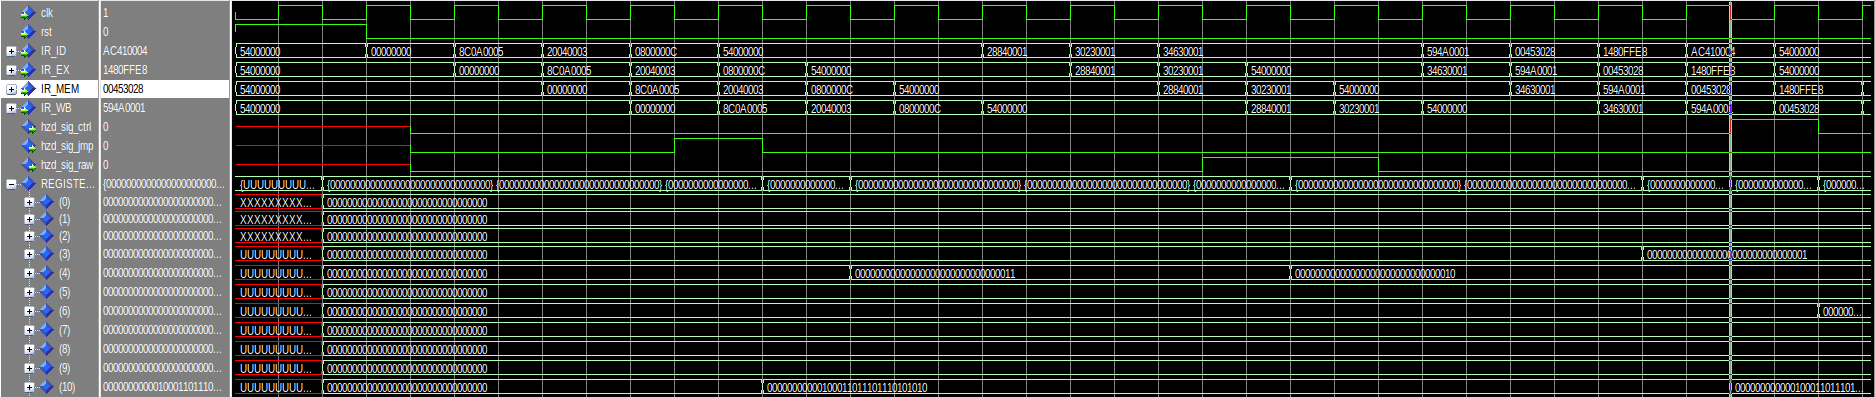
\includegraphics[width=\textwidth]{chapters/figures/waveform.png} 
	\caption{Modelsim waveform}
	\label{fig:wave}  % here is the figure label
	\end{figure}





